\chapter{System}

This chapter contains the state-of-the-art of the system, the design of the application architecture, the design of the scanning methodology, and the description of the Agile method used to develop the application.

% •	Description of the application architecture suitable for security scanning (executable, terminal, later ui)
  % o	System Settings UI and API to control every aspect of the device
% •	Agile method, stories, backlog

% Go language
% IEC62443 findings and table
% Explanation of the libraries used (Cobra for CLI, Zerolog for logging) and their benefits
% •	Design of the scanning methodology.
  % o	Aspects covered: Outdated OS, outdated libraries (e.g., OpenSSL), outdated software, default or weak credentials, insecure network communication, …

\section{Initial design}

As a reminder, the internship's company designs and builds industrial devices, as PLC or HMI. Under the hood, every PLC is powered by a custom Linux distribution, provided by \textit{Yocto Project}, an open source collaboration project that helps developers create custom Linux-based systems regardless of the hardware architecture~\cite{yocto-project}, that is developed by the internal \textit{Research \& Development} (R\&D) team.

In order to be able to make the device interacting with the industrial machines, the company provides a proprietary IDE software, needed to scratch projects and deploy them on the device. This software let the user define the inputs and outputs of the device, and the logic that will be executed on the device. In example, the user can define a trigger, an alarm that will be raised when a certain condition is met, a personalized handling of the data received by the many supported protocols, and so on.

Furthermore, the same IDE is used to draw the graphical interface that will be displayed on the HMI, and to define the behavior of the interface itself.\\
The graphical interface is composed by widgets, that are the building blocks of the interface. The user can define the position of the widgets, their size, their color, and their behavior. The widgets can be buttons, labels, images, graphs or custom-defined ones.

The setup with their IDE software is strictly related to the device interacting with the industrial machines, and it is not the focus of the internship project. The focus is on the device itself, and on the software that runs on it. \\
Another company of the group is in charge of the development of a management software that allows these devices to become domotic, that is industrial automation, in order to send and receive data from the cloud, to be able to interact with the device remotely, and to be able to monitor the status of the device. The software is a built-in service running on the hardware, and all the data are collected and sent to the cloud through the company's servers.

Given that, at the beginning, our scanning tool cannot be installed and released as a firmware update for the devices, because that would require a modification of the R\&D team's workflow, we decided to develop the scanning tool as an executable binary that can be run on the device itself. It is a \textit{command-line interface} (CLI) tool able to perform the scan and to report an output to the user. Than, the user will be able to fix the issues by itself, by interacting with the device settings.

\section{Device settings}

The PLC backend provides a web interface that can be used to view and change the system settings of the device. The user can change the network settings, set the datetime, set the management user password, manage the startup of the services like the SSH server, and much more. The HMI touchscreen, through dedicated gestures, let the user directly interact locally with the on-board interface, otherwise it is possible to reach it by connecting to the device's network address. \\
Client and server, respectively the graphical interface and the backend, are indipendent of each other; the web interface is powered by REST APIs, which are endpoints that can be called in a RESTful way, meaning that the user transfers a representation of the state of the resource to the requester or endpoint with appropriate HTTP methods to perform standard database functions like creating, reading, updating and deleting records (also known as \textit{CRUD}) within a resource.~\cite{rest-api}

For the internship project we will take advantage of the REST APIs to retrieve the status of the device, and to potentially change its settings. Internally to the company, the APIs are documented with the \textit{OpenAPI Specification}, formerly \textit{Swagger Specification}, that is an API description format that depicts the endpoints, the parameters, the responses, the authentication needed to call them and licenses or other informations. The Swagger file can be visualized through the Swagger UI, a web interface that renders OpenAPI definitions as interactive documentation.~\cite{openapi-swagger}

We can devise two different scenarios: API calls made by a remote host over a network and API calls made by the local host. In the first case, the TLS protocol secures the communication using the public-key authentication first, and then the APIs are protected by a basic authentication, that is the client must provide a management username and its related password. In the second case, the webserver listens over a port only accessible by the same host with no further authentication needed. 
% TODO: Note about use-cases and security of this approach

\section{\textit{Go} programming language}

\textit{Go} is an open-source programming language supported by Google, designed for building simple, reliable, and efficient software. It is statically typed, compiled, and syntactically similar to C, with the added benefits of built-in concurrency management, garbage collection, memory safety, and a robust standard library plus packages. Go is widely used in cloud computing, web development, and systems programming due to its simplicity, performance, and scalability.~\cite{go-lang-site}~\cite{go-lang-wikipedia}\\
Go has been released in 2007 by Google, and at the time of writing it is at version \texttt{1.22}.

One of the main reasons for choosing Go for the internship project is its versatility in building executable binaries for multiple platforms, including Windows, macOS, and Linux. Go's cross-compilation capabilities allow the developers to build binaries for different operating systems and architectures from a single codebase, simplifying the deployment process and ensuring compatibility across various platforms. Given that the industrial devices run on different architectures and operating systems, the ability to build cross-platform binaries is essential. The language natively supports the binaries compilation for over 50 combinations of operating systems and architectures~\cite{go-lang-compilation-combo}; given that the majority of the company's devices run either on \texttt{Arm 32bit} or \texttt{Arm 64bit} or \texttt{x86 64bit} architectures, the Go compiler can generate the executables for these architectures with no further configuration needed.

Go's standard library provides comprehensive support for networking, encryption, and concurrency. The built-in packages for HTTP, TLS, and JSON processing simplify the implementation of RESTful APIs, secure communication channels, and data serialization/deserialization, respectively. If additional functionalities are required, the language supports third-party packages through the Go module system; in order to download a custom package, the developer simply reference it in the code via the link to the repository, and the Go compiler will automatically download and install it.

Go also offers a robust testing framework to write unit tests and benchmarks to ensure the reliability and performance of their code. The testing framework is integrated into the language and provides a simple and efficient way to write tests for functions and methods. The testing framework also supports the generation of code coverage reports to identify untested code paths and improve the overall test coverage. Furthermore, Go's testing framework supports the use of table-driven tests, which allow the developer to define test cases in a structured format and iterate over them to execute the tests and also it supports fuzzing, a technique used to discover vulnerabilities in software by providing random or invalid inputs to the program.

Another point in favor is the efficiency of the language. Go is compiled to machine code, which makes it faster than interpreted languages like Python. The language's garbage collection mechanism automatically manages memory allocation and deallocation, reducing the risk of memory leaks and improving the overall performance of the application. The language is more than a full order of magnitude faster than Python, with a smaller memory footprint and faster execution times.~\cite{go-lang-performance}

\section{How IEC 62443 driven the design}

Recalling~\cref{sec:iec-62443}, the IEC 62443 standard provides a comprehensive framework for securing industrial control systems and operational technology networks. In order to perform a step towards the certification of the devices with the standard, the scanning tool must cover at least the aspects of the standard.

We did a case-study on the standard documentation: for each of the security requirements listed in the \texttt{3-3}, \texttt{4-1} and \texttt{4-2} documents, we said: 
\begin{mdframed}
  \textit{\textless\textless  Can we implement a check for this requirement in such a way to make the user able to fix the potential issue by itself? \textgreater\textgreater}
\end{mdframed}
We considered the user as a person that has a management account on the device, and that has to interact using the settings web interface. The goal was to make the final user able to fix the reported issue without the need of updating the firmware or asking for a modification on the source-code or on the development lifecycle.

\cref{fig:iec62443-findings-3_3} and~\cref{fig:iec62443-findings-4_2} show the findings of the case-study. The table is divided into four columns: the first one is the security requirement title, the second one is the description text, the third is whether we believe that it is a check we should implement on a scanning tool and the fourth one contains some notes about the possible implementation.

\begin{figure}[t]
  \centering
  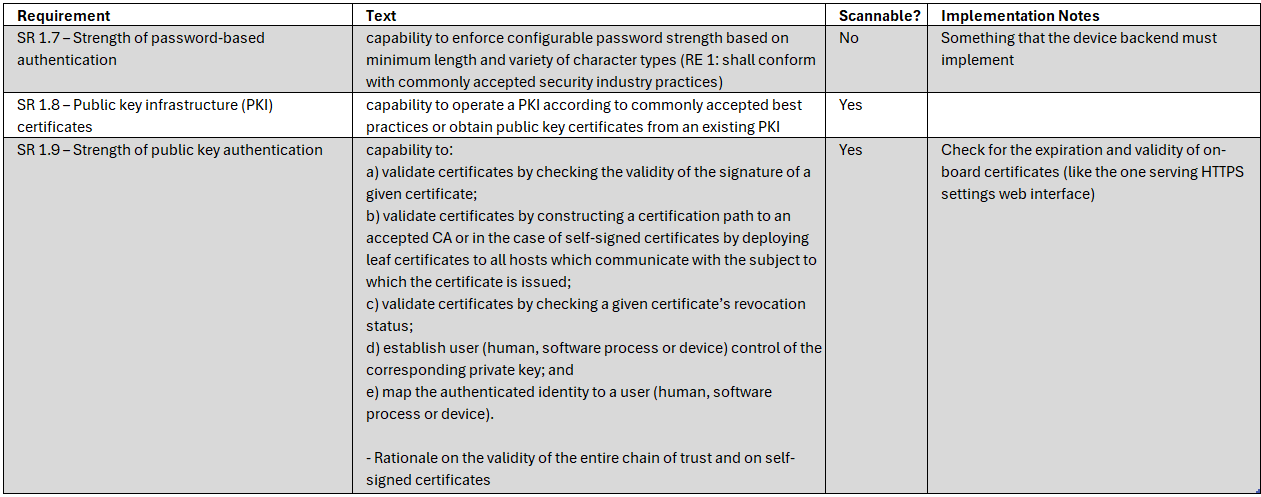
\includegraphics[width=1.0\textwidth]{chapters/04/assets/iec62443-findings-3_3}
  \caption{IEC 62443 \texttt{3-3} chosen requirements}
  \label{fig:iec62443-findings-3_3}
\end{figure}

\begin{figure}[t]
  \centering
  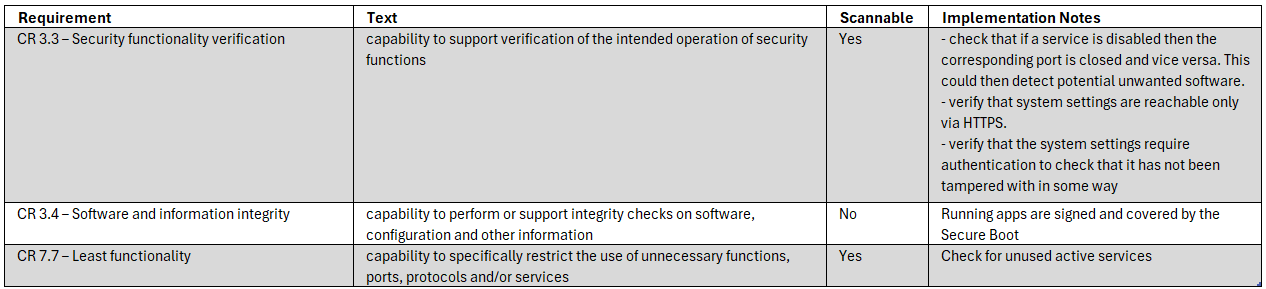
\includegraphics[width=1.0\textwidth]{chapters/04/assets/iec62443-findings-4_2}
  \caption{IEC 62443 \texttt{4-2} chosen requirements}
  \label{fig:iec62443-findings-4_2}
\end{figure}

To better explain our choices and motivations, we now take into account the \textit{SR 1.9 - Strength of public key authentication} requirement. The requirement states that there must be the capability to validate the validity of the used certificates by checking the signature, the expiration date, and the revocation status. We believe that this is a check that we should implement in the scanning tool, because the user can fix the issue by itself by renewing the certificate, or by changing the certificate authority if needed. The implementation of the check could be done by retrieving the certificate from the device, and then checking the signature, the expiration date, and the revocation status. If the certificate is self-signed, the tool could suggest the user to change it with a certificate signed by a trusted certificate authority.

Instead, we now consider the \textit{SR 1.7 - Strength of password-based authentication}. The requirement states that the password must have a minimum length and variety of characters types. We put this assertion in a limbo, because if the user can set a password not respecting the requirement, the tool, which is an intermediate between the user and the backend, cannot enforce the requirement. Than, the issue should be solved by the R\&D team, that should implement a password policy on the backend, and the user should be forced to change the password at the next login.

With this approach, we have identified the checks that the scanning tool should cover for sure from the standard, and we have included them in the backlog of the project.

